
\subsubsection{Proposed approach for $W\rightarrow\ell\nu$ analysis at 13~TeV}
\label{sec:bkg_mj_approach}

A possible solution to some of these problems is used in Ref. \cite{Andari:1976186}: several MJ-templates are defined slicing the lepton isolation variable for values greater than the one used in the SR and progressively farther from the SR lepton selection.
The MJ extraction fit on a kinematic variable is then repeated for each of the MJ-templates corresponding to each slice. 
The result is a “scan” of the MJ extractions with templates closer and closer to the SR lepton selection.
It is then possible to linearly extrapolate the MJ estimate into the signal region.
This procedure addresses the following points:
\begin{itemize}
\item the MJ-template selection is not arbitrary any more, in fact ideally the MJ estimate coming from the extrapolation is the one with the SR selection;
\item the biases in the kinematic or in the composition of the MJ-template reduce as the MJ-selection gets closer to the SR selection;
\item different variables are used in the MJ-extraction fits, and the MJ extrapolation is repeated for each of them.
\end{itemize}

\todo{MJ fit formula here}

One not trivial point in the definition of the scan is the choice of the variable to slice on for the MJ-template building. 
% We investigated the option of using Lepton-ID based variables, as the electron-ID likelihood value. 
% However this was not feasible because of the need of low statistics pre-scaled support trigger for the MJ-template selection, the multi-dimensional optimization used to build the electron-ID likelihood selection, and the poor statistics available in the loose-not-medium electron sample. 
% Therefore 
We decided to invert the isolation selection for the construction of the MJ templates, keeping the rest of the selection cuts like the nominal signal selection.
This revealed not to be straightforward because this analysis uses the ``Gradient-Iso'' working point to define a lepton as isolated or not.
The Gradient-Iso selection is a $p_T - \eta$ dependent cut on both calorimeter and track relative isolation variables: ptvarcone20(30)/$p_T$ and topoetcone20/$p_T$ for electrons (muons).

We decided to scan both the isolation variables to cover for the different effects which may come from the inversion of the calorimeter or track isolation. 
The scan slice size and interval have been identified by analysing the ptvarcone20(30)/$p_T$ versus topoetcone20/$p_T$ distributions for electrons (muons) in data for events passing or failing the Gradient-Iso selection.
The result is reported in Fig.\ref{fig:isolation_2D}.
The events passing the Gradient-Iso cut appear to be bounded in the regions:
\begin{equation}
  \label{eq:XvarConeSRCuts}
  \frac{ptvarcone20(30)}{p_T} <0.06~(0.11)~\&\&~\frac{topoetcone20}{p_T} <0.13~(0.09)
\end{equation}
for electrons (muons).
Given the particular phase-space defined by the Gradient isolation requirement, (the definition of the isolation criteria depends on $p_T$ and $\eta$ of the lepton) we decided to produce MJ-templates inverting the Gradient isolation requirement but only considering the events outside the area delimited by Eq. \ref{eq:XvarConeSRCuts}. 
This forces the extrapolation from a region not immediately adjacent to the SR lepton selection, and is an intrinsic problem of the use of the Gradient-Iso selection.

\begin{figure}[htbp]
\centering
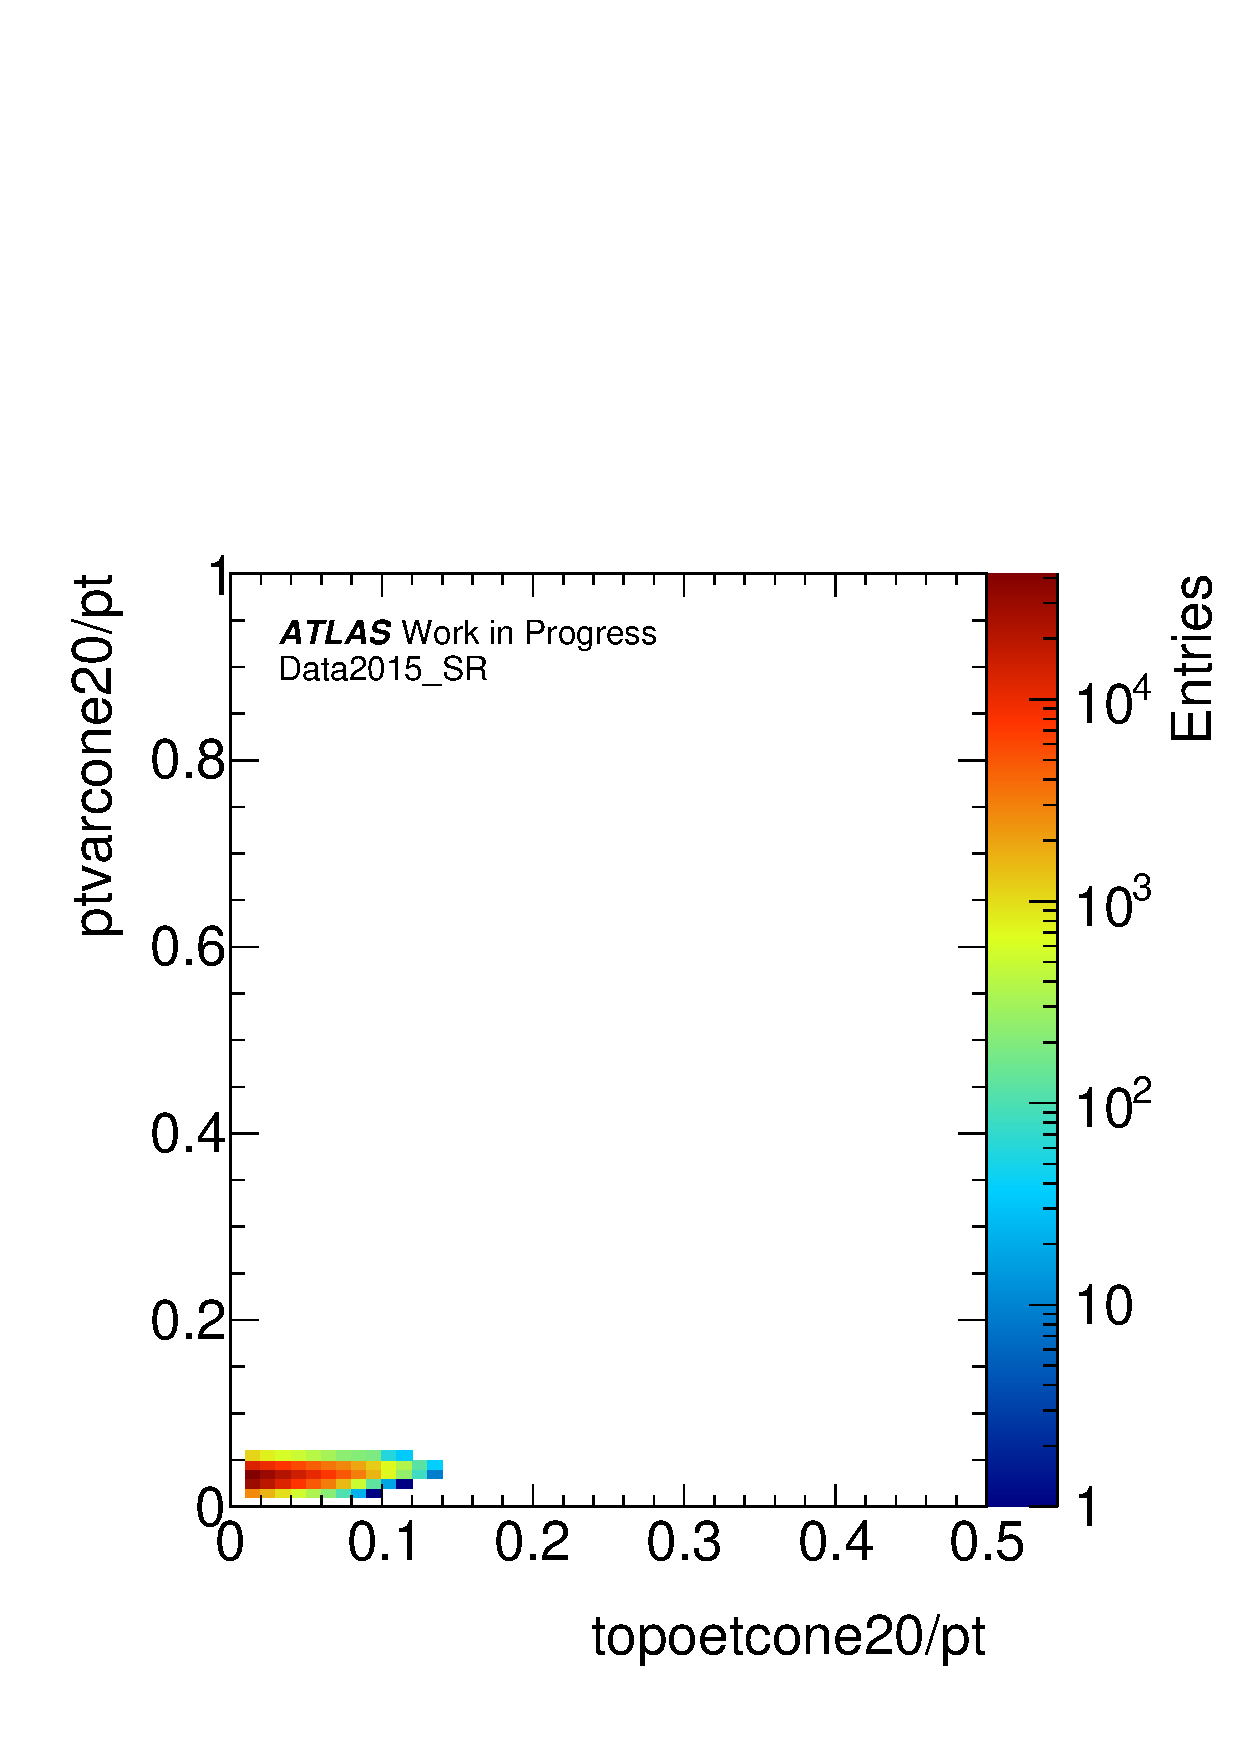
\includegraphics[width=0.4\textwidth]{figures/mj/plot2D-Data2015_SR-el_lep_0_iso_topoetcone20dPtVSel_lep_0_iso_ptvarcone20dPt-el.pdf}
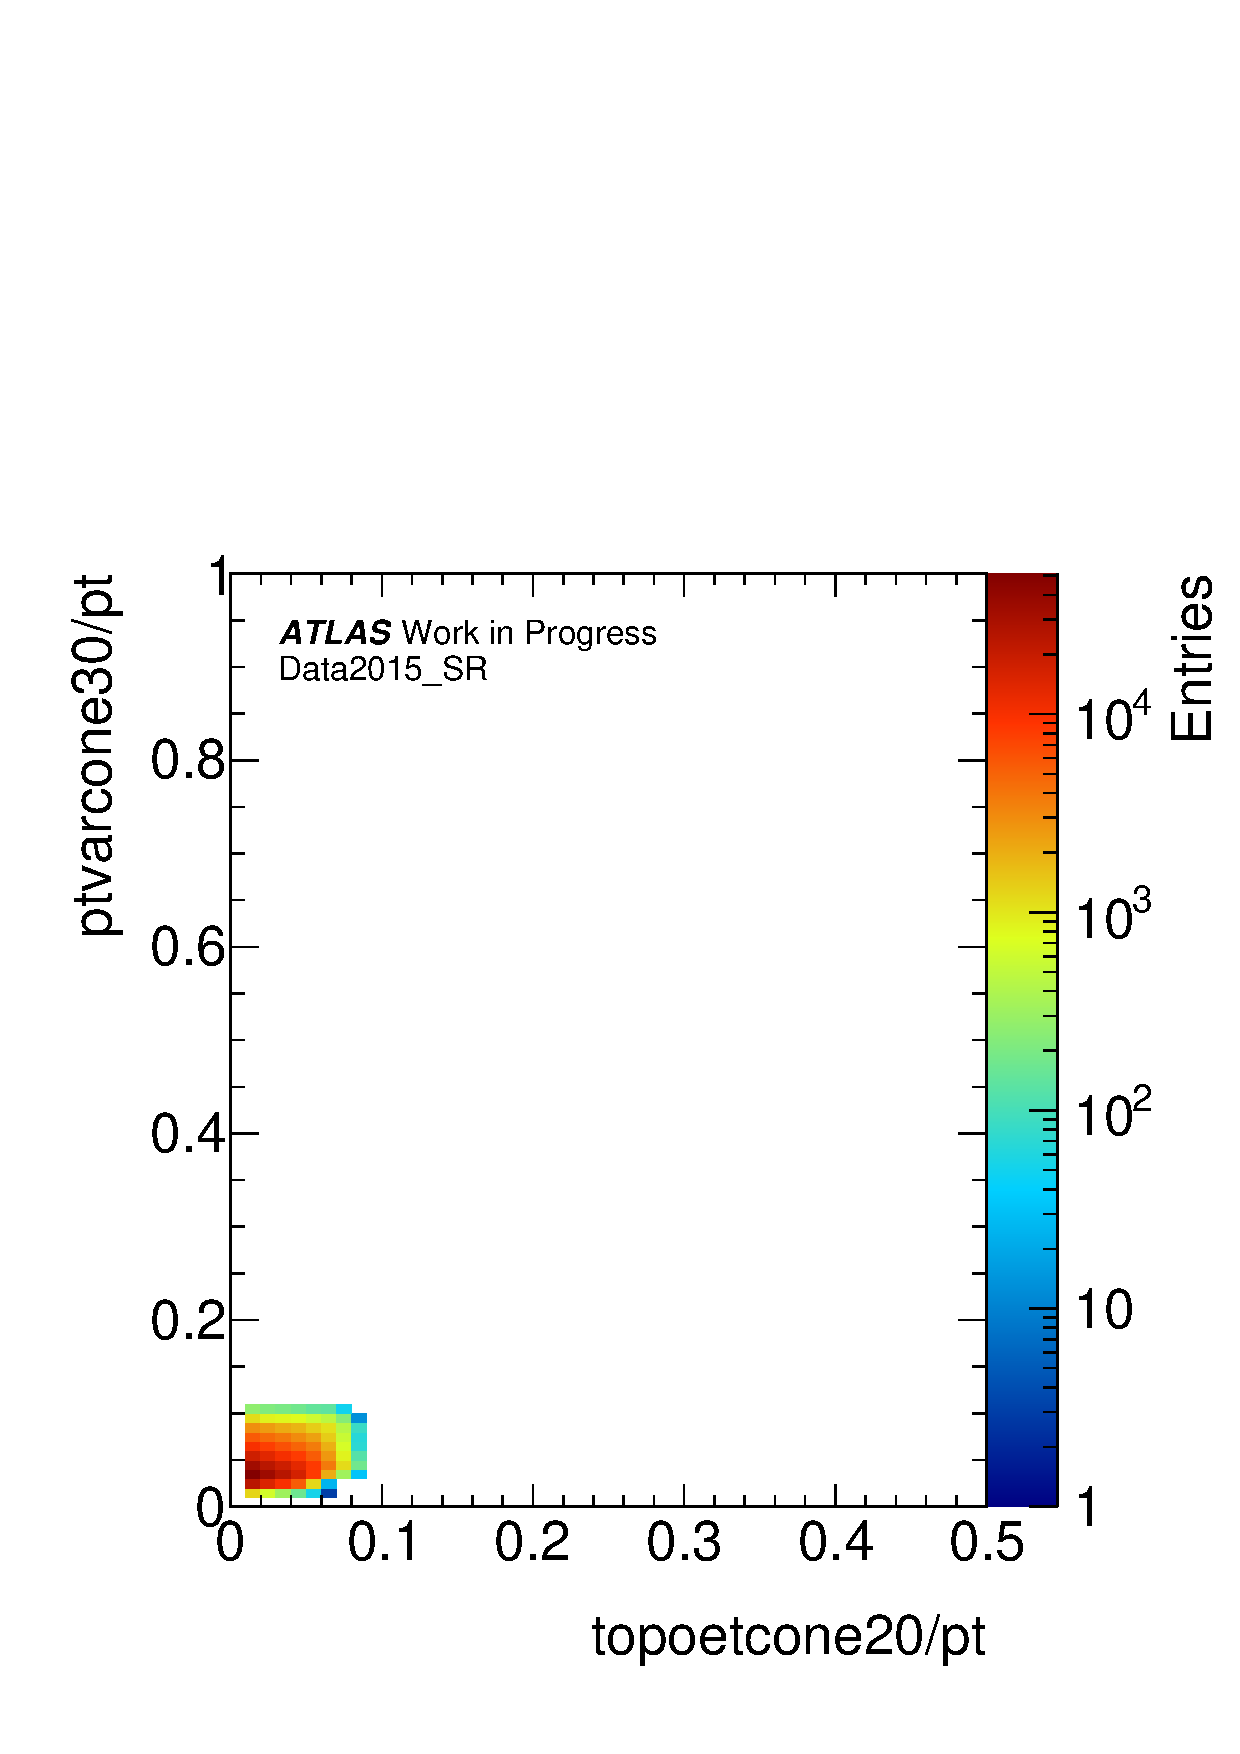
\includegraphics[width=0.4\textwidth]{figures/mj/plot2D-Data2015_SR-mu_lep_0_iso_topoetcone20dPtVSmu_lep_0_iso_ptvarcone30dPt-mu.pdf}
\\
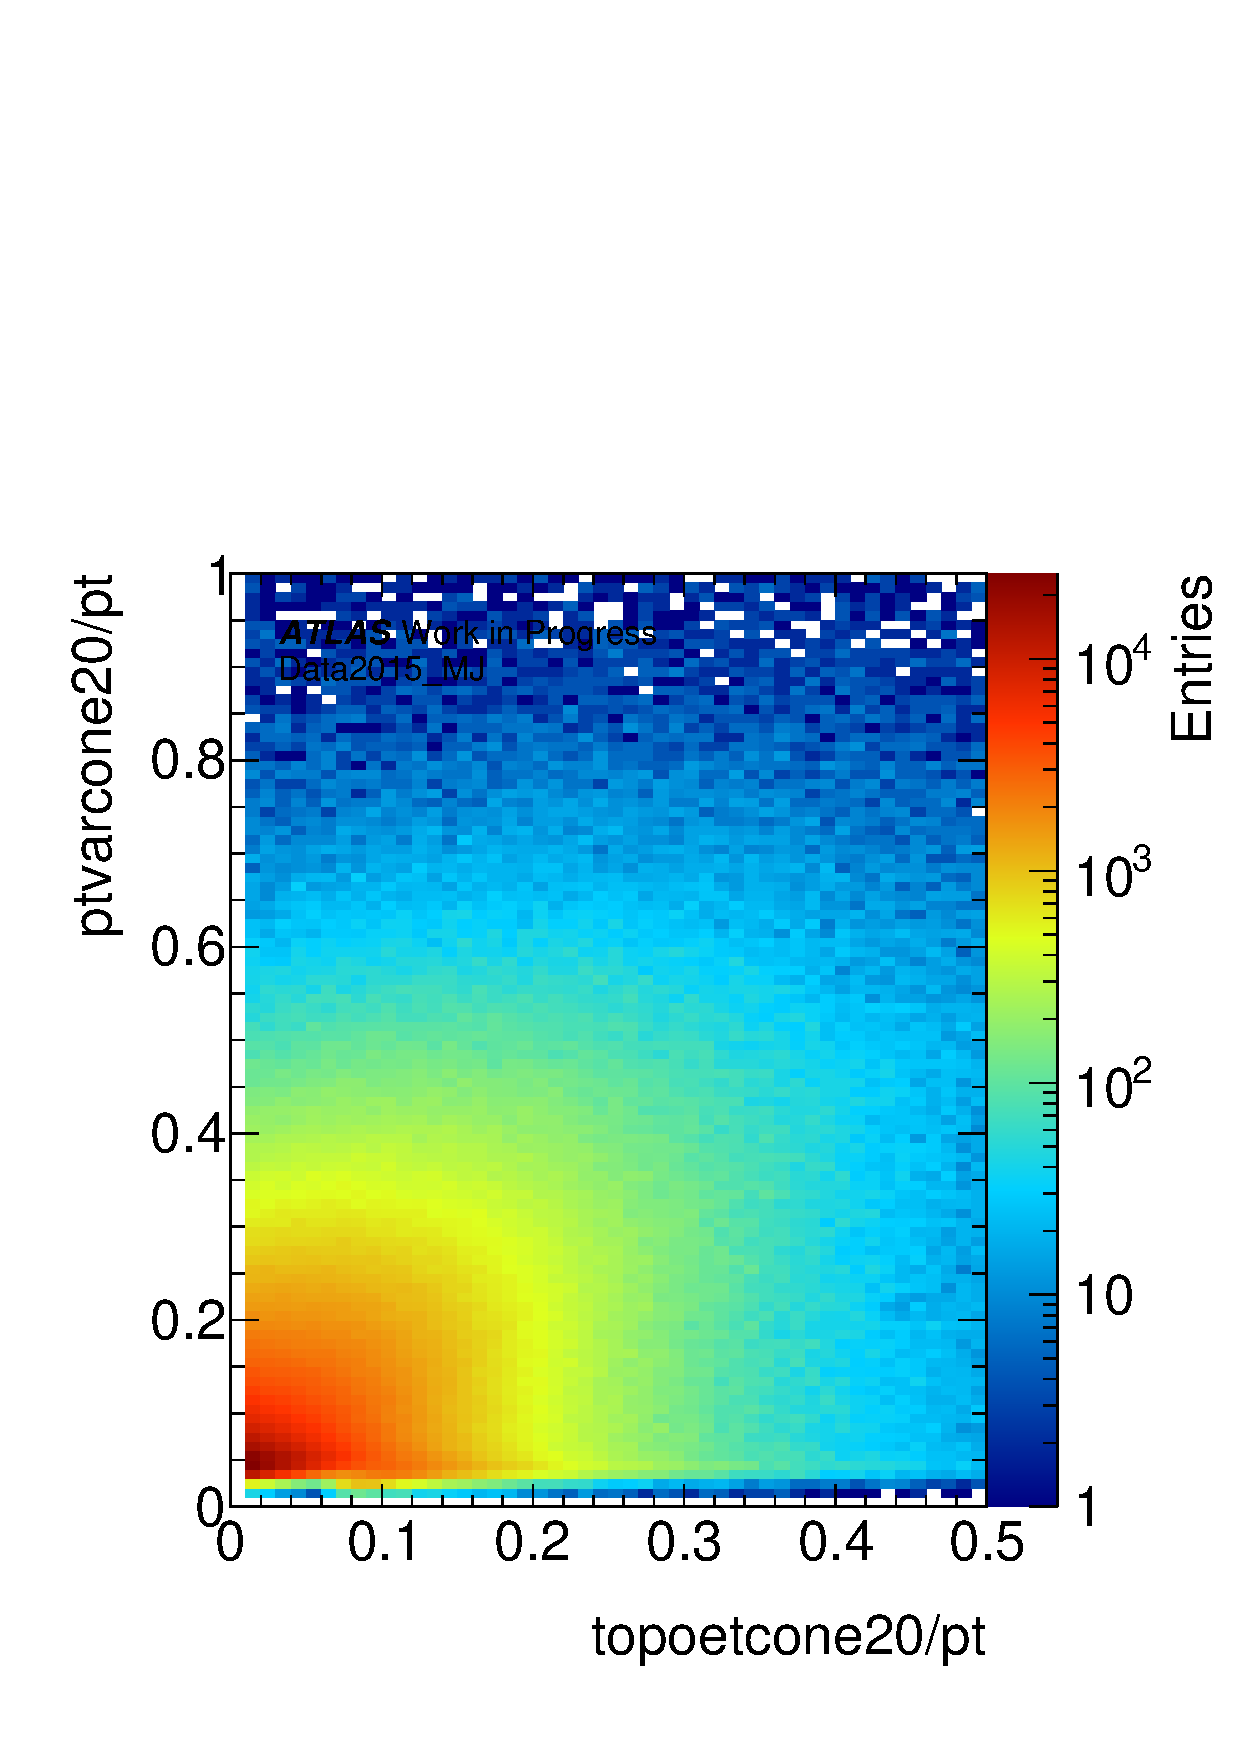
\includegraphics[width=0.4\textwidth]{figures/mj/plot2D-Data2015_MJ-el_lep_0_iso_topoetcone20dPtVSel_lep_0_iso_ptvarcone20dPt-el.pdf}
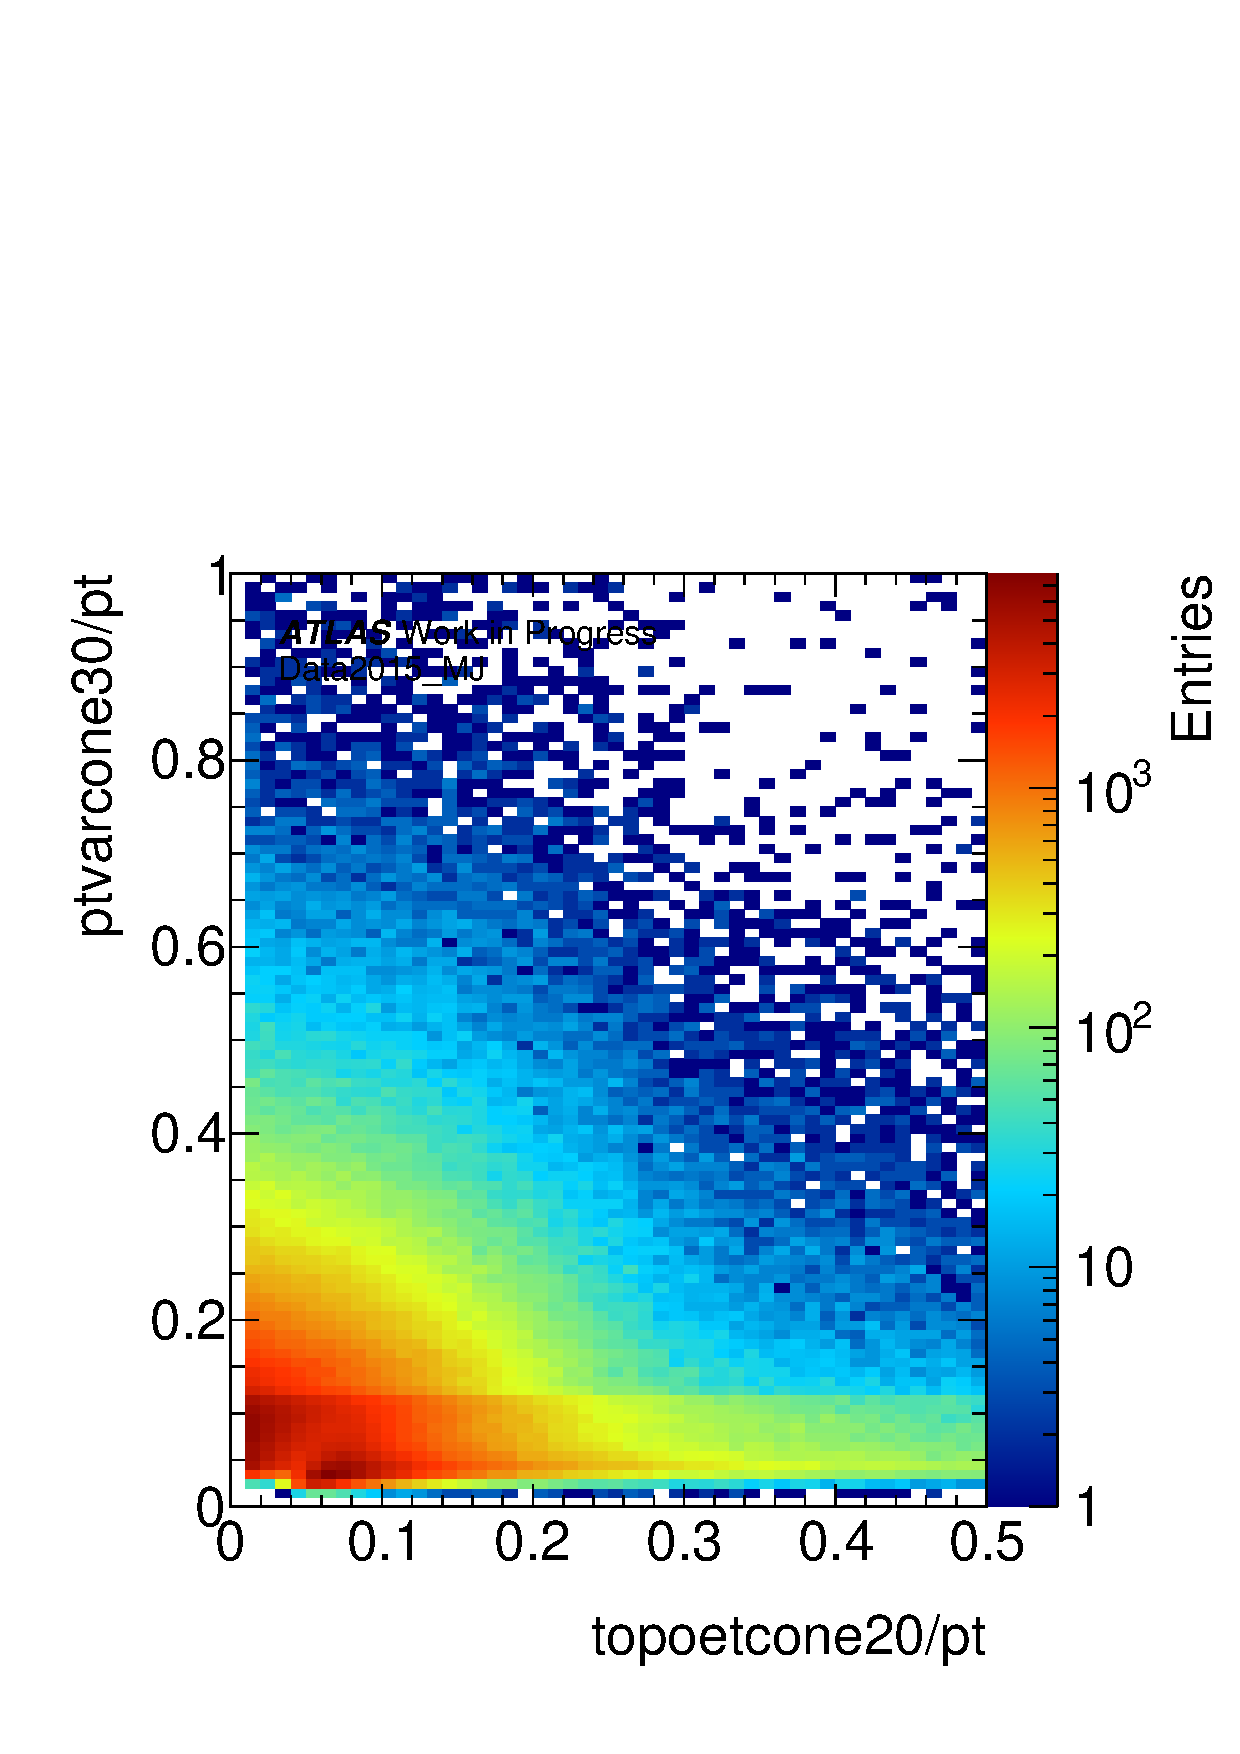
\includegraphics[width=0.4\textwidth]{figures/mj/plot2D-Data2015_MJ-mu_lep_0_iso_topoetcone20dPtVSmu_lep_0_iso_ptvarcone30dPt-mu.pdf}
\caption{
 Distribution of ptvarcone20(30)/$p_T$ versus topoetcone20/$p_T$ for electrons (left) and muons (right) for events passing (top) or failing (bottom) the Gradient-Iso selection in the data.
}
\label{fig:isolation_2D}
\end{figure}

As the Gradient-Iso phase space is only in a rectangular region of ptvarconeXX/$p_T$ versus topoetcone20/$p_T$, we decided to scan in slices of one isolation requirement at the time applying a fix cut on the other requirement to avoid biases from very non isolated events. 
The distribution of events failing the Gradient-Iso selection shown in Fig. \ref{fig:isolation_2D} gives also indication of the possible scan range and statistics of the scan  slices.

The fit was performed in two separate regions (fir regions - FR’s) defined removing in one case the $m_T^W > 40$ GeV cut, and in the other case removing the $E_T^{miss} > 25$ GeV cut.
In each fit region, fits are performed on following four variables: $p_T^{\ell}$, $E_T^{miss}$, $m_T^{W}$ and $\Delta \varphi _{\ell,E_T^{miss}}$ for each of the scan points, and the fraction of MJ is estimated extrapolating back to the signal region (re-applying the $m_T^W > 40$ GeV cut in one case, and the $E_T^{miss} > 25$ GeV cut in the other).
The contamination in each of the template regions, coming from the signal and the EW+top backgrounds varies a lot depending on the scan region.
A detailed description of such contaminations is reported in Table \ref{tbl:mj_ewk_bkg_fraction} and \todo{54}.

The stability of the MJ extraction was checked in several ways: the width of the \todo{isolation scan slices was varied}, the variables were fit in \todo{reduced ranges of the histograms} to reduce the impact of mismodellings of the data/MC distributions, and the EW and top backgrounds were \todo{kept fixed} by considering a very small Gaussian constraint on them.
In all these tests, the MJ estimates scans \todo{resulted to be close to one another}, and significantly smaller than the spread in the extrapolation coming from the use of different fit variables.
The study corresponding to a variation of the normalisation constraint on the EWK and top background is documented in detail in \todo{Appendix K}.

\subsubsection{$W\rightarrow e\nu$ scan results}
\label{sec:bkg_mj_we_scan}

As discussed in Sec. \ref{sec:bkg_mj_approach}, the events passing the gradient isolation cut and the selection are confined in the region of ptvarcone20/$p_T$ < 0.06 and topoetcone20/$p_T$ < 0.13. 
For this reason scans on the two variables,after inverting the gradient isolation, are performed for the values reported in Table \ref{tbl:mj_scan_binning_el}.

\begin{table}[htbp]
\small
\begin{center}
 \begin{tabular}{ | c | c | c | } 
 \hline
 Scan variable & ptvarcone20/$p_T$ & topoetcone20/$p_T$ \\
 \hline 
 Fixed cut & topoetcone20/$p_T$ < 0.13 & ptvarcone20/$p_T$ < 0.06 \\
 \hline 
 Scan starting point & 0.06 & 0.13 \\
 Slice width & 0.09 & 0.045 \\
 Number of slices & 6 & 6 \\
 \hline 
\end{tabular}
\caption{
Width of scan slices and boundaries used for $W\rightarrow e\nu$ channel.
}%
\label{tbl:mj_scan_binning_el}
\end{center}
\end{table}

The results for topoetcone20/$p_T$ and ptvarcone20/$p_T$ scans, and in the two fit regions, performed on $E_T^{miss}$, $m_T$, $p_T$ and $\Delta\varphi_{e,E_T^{miss}}$ are reported in Fig.\ref{fig:mj_extrapolation_wenu} for the $W\rightarrow e\nu$ channel.
Notice that the $\Delta\varphi_{e,E_T^{miss}}$ variable is missing $E_T^{miss}$-FR scans because returning often nonphysical negative or zero MJ yiels because of the poor discrimination power of such variable after the $m_T$>40 GeV cut is applied.
The errors on each of the scan points are the errors from the template fit, taking into account the discrimination power of the variables, as well as the statistics of the MJ template, \todo{multiplied by the $\sqrt(\chi^2/NDoF)$}, to account for eventual mismodelling in the considered variables.
More details on the extraction of the numbers are reported in Appendix \ref{sec:details_on_multijet_background_estimate_in_the_Wenu_channel}.

\begin{figure}[htbp]
\centering
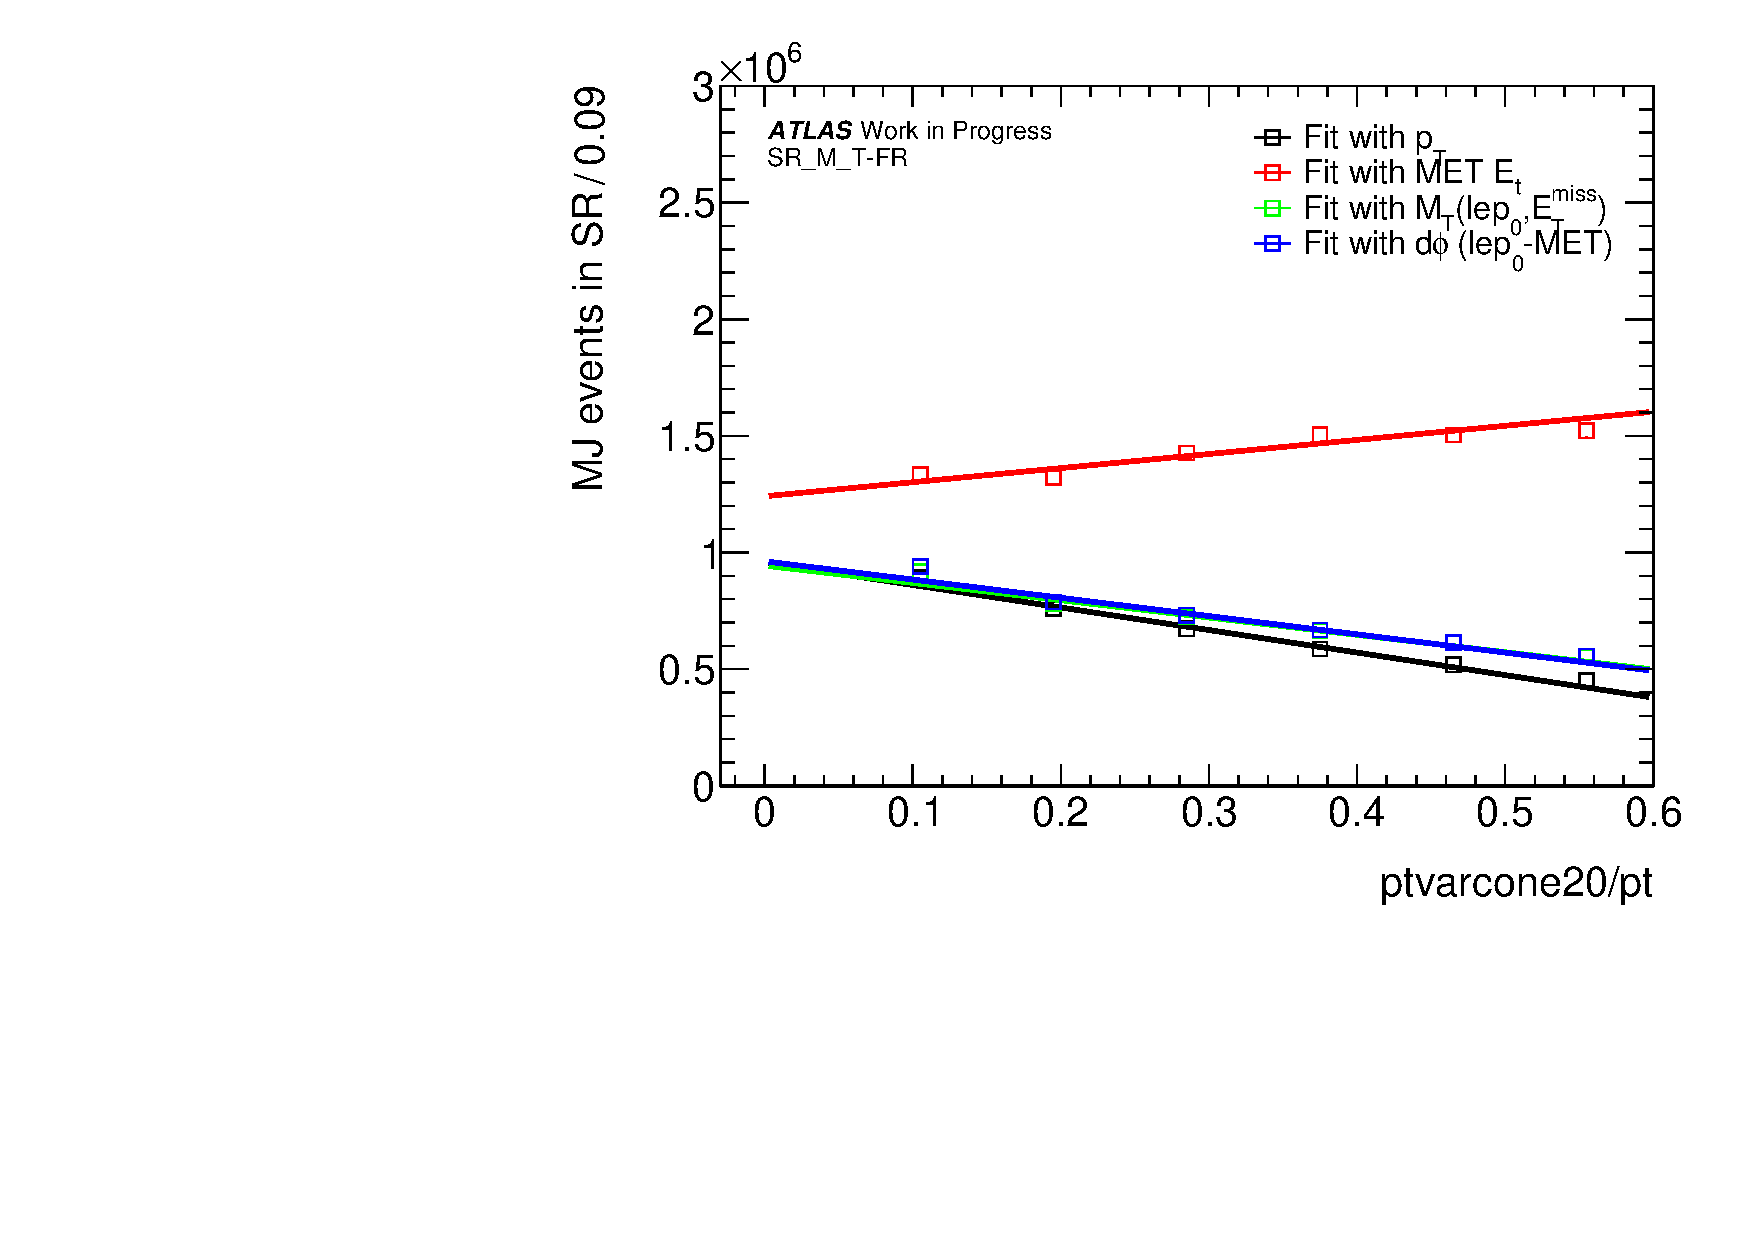
\includegraphics[width=0.45\textwidth]{figures/mj/slicesScanFit_SR_M_T_ptvar_el.pdf}
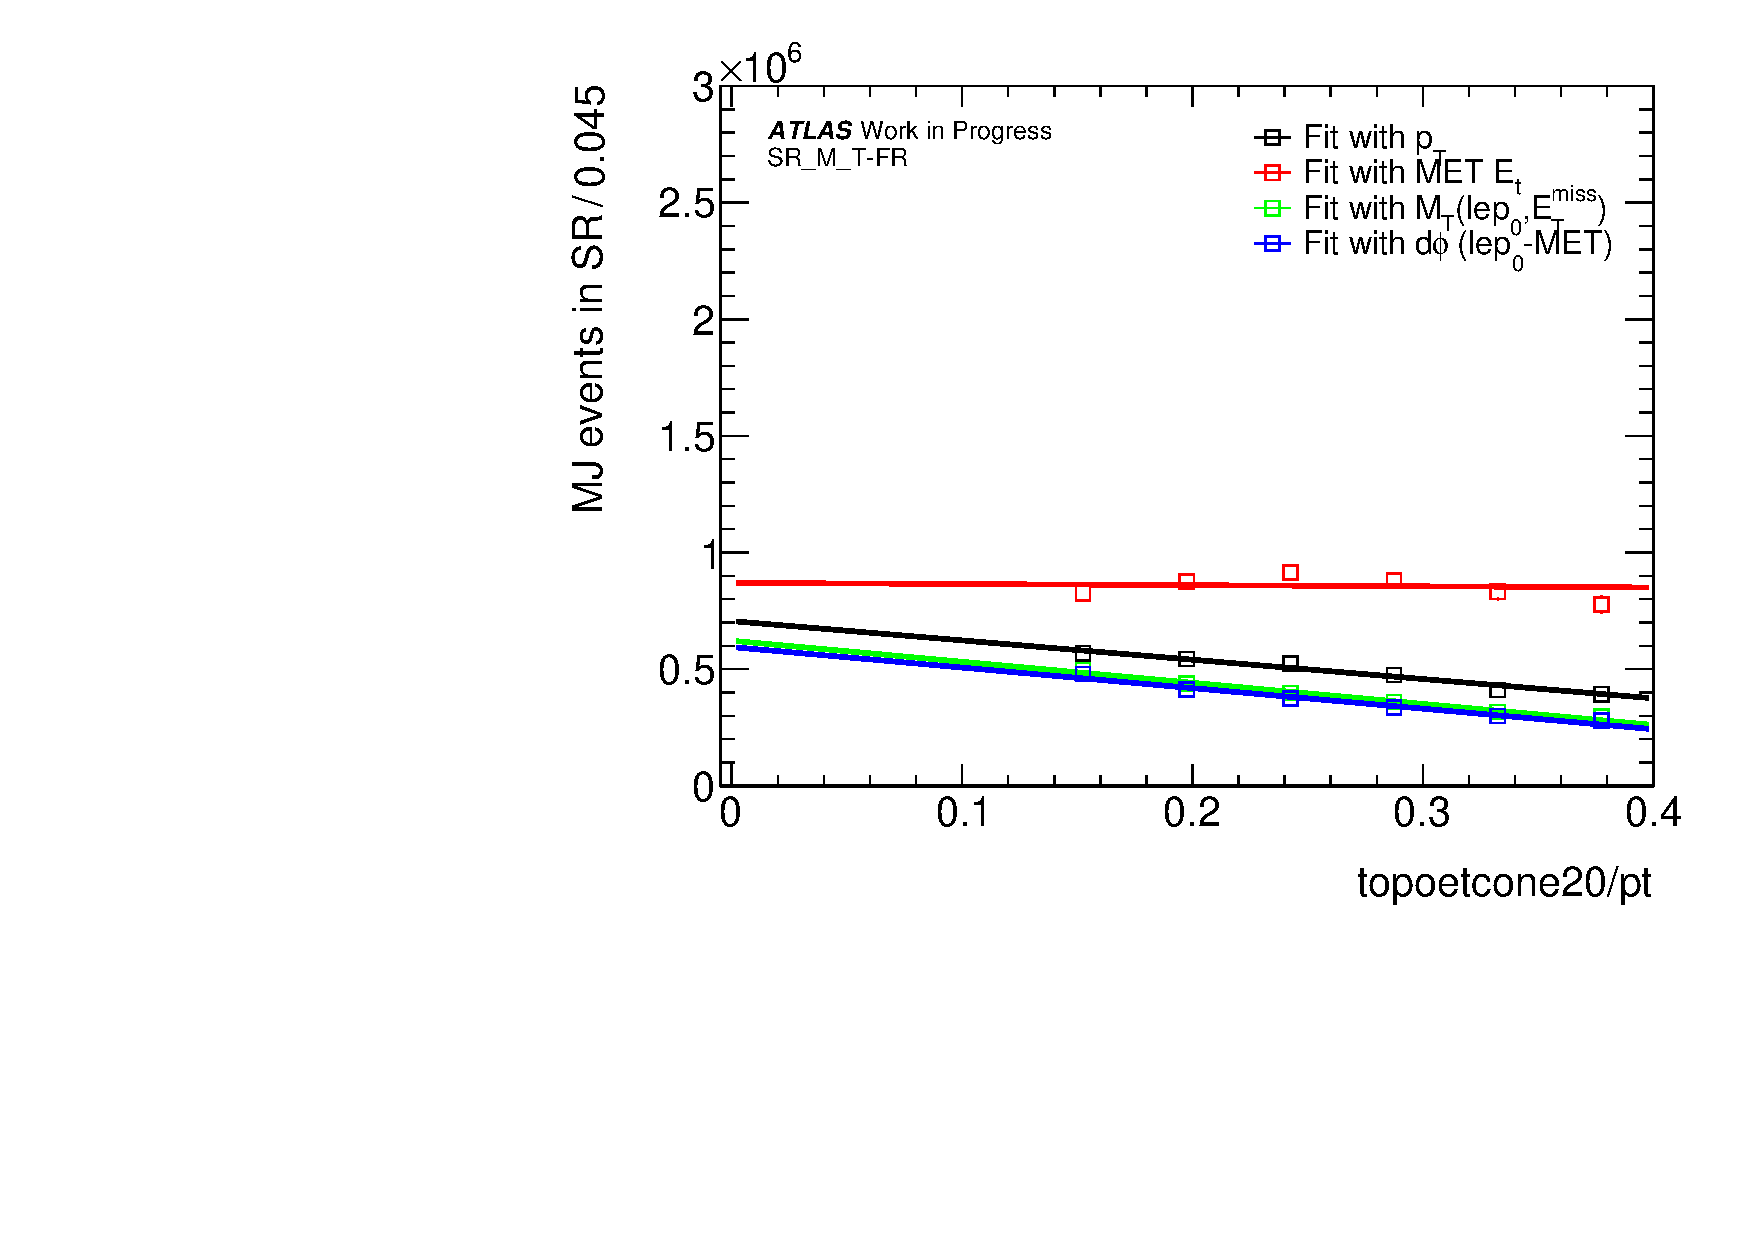
\includegraphics[width=0.45\textwidth]{figures/mj/slicesScanFit_SR_M_T_topoet_el.pdf}
\\
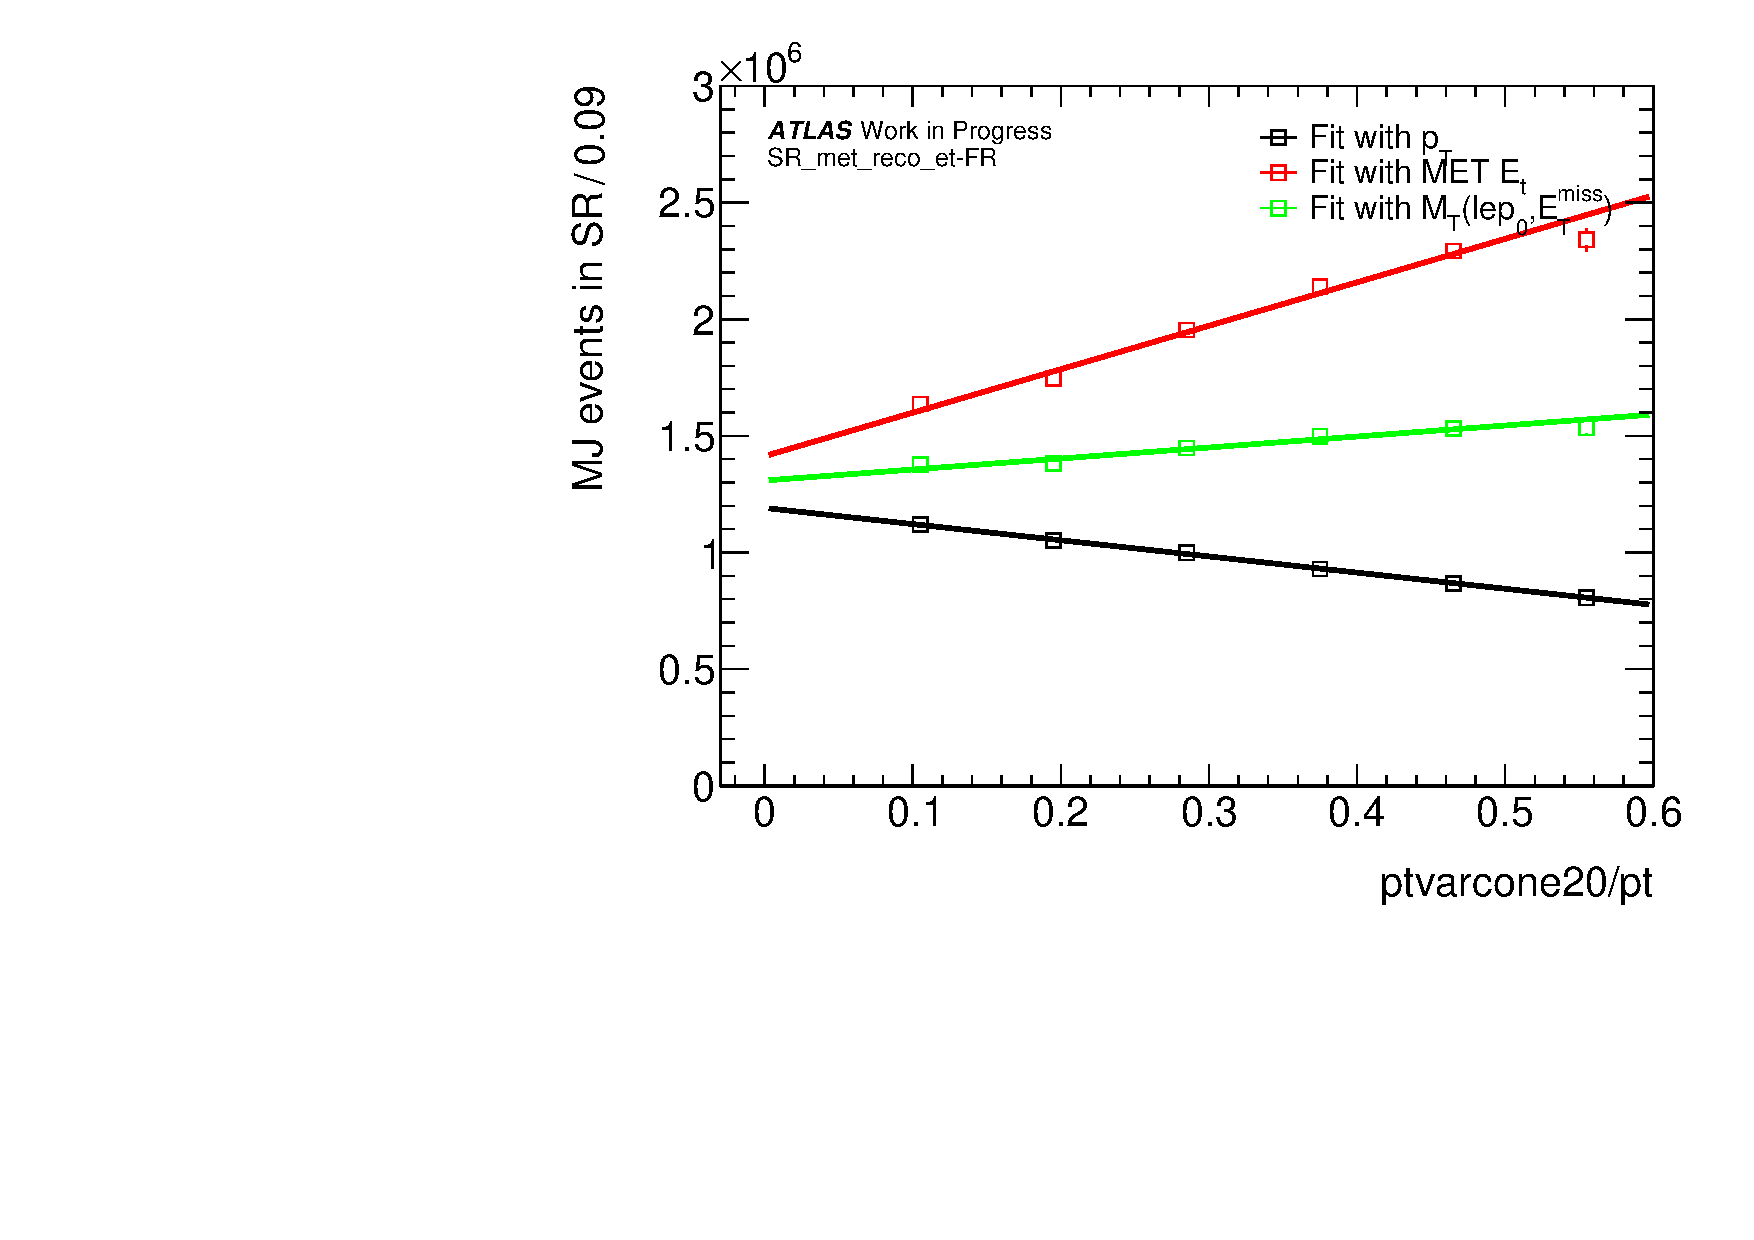
\includegraphics[width=0.45\textwidth]{figures/mj/slicesScanFit_SR_met_reco_et_ptvar_el.pdf}
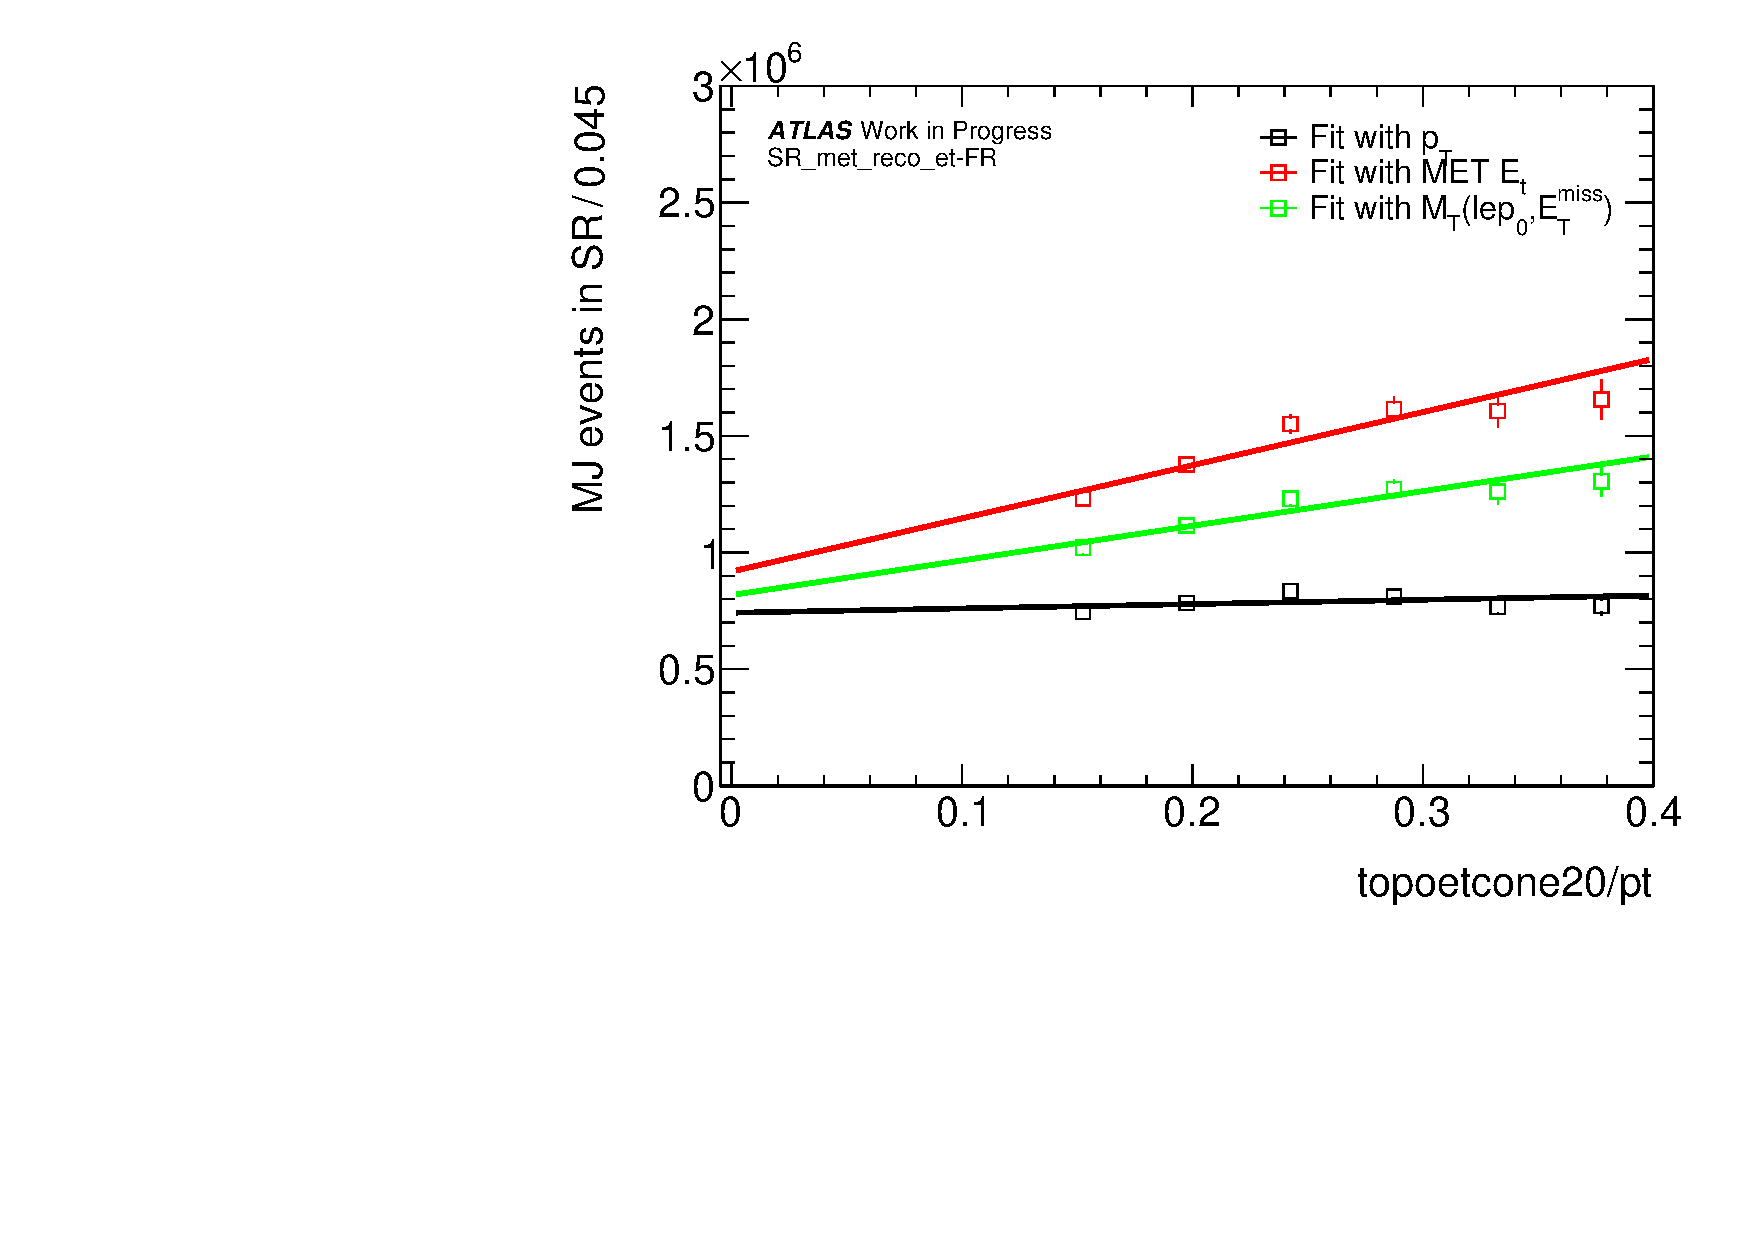
\includegraphics[width=0.45\textwidth]{figures/mj/slicesScanFit_SR_met_reco_et_topoet_el.pdf}
\caption{
 Plots of the scans for ptvarcone20/$p_T$ (left column) and topoetcone20/$p_T$ (right column) for the $W\rightarrow e\nu$ channel, $m_T$-FR (top raw), $E_T^{miss}$-FR (bottom row).
 The results relative to the scans of the different variables (fit in each slice and linear extrapolations) are shown in different colors: $E_T^{miss}$ (blue), $m_T$ (green), $p_T$ (red) and $\Delta\varphi_{e,E_T^{miss}}$ (black).
 Notice that the $\Delta\varphi_{e,E_T^{miss}}$ variable is missing $E_T^{miss}$-FR scans because 
 returning often nonphysical negative or zero MJ yiels because of the poor discrimination power of such variable after the $m_T$>40 GeV cut is applied.
 The errors on each of the scan points are the error from the template fit \todo{multiplied by the $\sqrt(\chi^2/NDoF)$}.
}
\label{fig:mj_extrapolation_wenu}
\end{figure}

In the plots it is visible the different behaviour of the variables, and their spread close to the signal region.
The fits performed on the $E_T^{miss}$ distribution have large error, coming mainly from the poor discriminating power of the $E_T^{miss}$.
Because of this the MJ extraction relative to the $E_T^{miss}$ has very large errors and central value relatively far from the one obtained with the other variables.
% The fits performed in the $E_T^{miss}$-relaxed fit region tend to \todo{give a slightly lower MJ estimate} with respect to the corresponding ones performed in the $m_T$-relaxed fit region.

The SR point of extrapolation is extracted from the average value of the ptvarcone20/$p_T$ and topoetcone20/$p_T$ distributions passing the gradient isolation selection cut in data (X and Y average of top left subfigure of Figure \ref{fig:isolation_2D}).
These values are \todo{0.034} and \todo{0.034} respectively.
The extrapolated values for $W\rightarrow e\nu$ for the topoetcone20/$p_T$ and ptvarcone20/$p_T$ respectively are reported in Table \ref{tbl:bkg_mj_we_scan_topoet} and \ref{tbl:bkg_mj_we_scan_ptvar}.
For details on the choice of the extrapolation values see \todo{Appendix P}.

\begin{table}[htbp]
\scriptsize
\begin{center}
 \begin{tabular}{ c | c  c | c  c } 
 \hline
Fit variable & MJ extrapolated SR\_met\_reco\_et-FR & $\chi^{2}$/NDoF of linear fit & MJ extrapolated SR\_M\_T-FR & $\chi^{2}$/NDoF of linear fit \\
\hline
\multicolumn{5}{c}{$W \rightarrow e \nu$} \\
\hline
$p_{T}$ & 741627.9 $\pm$ 34625.17 & 8.66/4 & 705913.9 $\pm$ 22912.59 & 3.99/4\\
$M_{T}(lep_{0},E^{miss}_{T})$ & 817560.7 $\pm$ 50581.89 & 5.95/4 & 621901.1 $\pm$ 18601.02 & 2.84/4\\
$d\phi (lep_{0}-MET)$ & - & -  & 594717.6 $\pm$ 17719.91 & 5.50/4\\
$MET E_{t}$ & 918511.4 $\pm$ 62436.09 & 8.67/4 & 869776.8 $\pm$ 37515.26 & 13.21/4\\
 \hline 
\end{tabular}
\caption{
Results of the extrapolation to the $W\rightarrow e\nu$ signal region (topoetcone20/$p_T$ = \todo{0.034}). 
The errors quoted come from the extrapolation at the SR points, varying in an anti-correlated way the $p_0$ and $p_1$ linear fit parameters of one $\sigma$.
}%
\label{tbl:bkg_mj_we_scan_topoet}
\end{center}
\end{table}

\begin{table}[htbp]
\scriptsize
\begin{center}
 \begin{tabular}{ c | c  c | c  c } 
 \hline
Fit variable & MJ extrapolated SR\_met\_reco\_et-FR & $\chi^{2}$/NDoF of linear fit & MJ extrapolated SR\_M\_T-FR & $\chi^{2}$/NDoF of linear fit \\
\hline
\multicolumn{5}{c}{$W \rightarrow e \nu$} \\
\hline
$p_{T}$ & 1191011.7 $\pm$ 7675.67 & 1.64/4 & 957321.2 $\pm$ 5624.70 & 57.39/4\\
$M_{T}(lep_{0},E^{miss}_{T})$ & 1308570.5 $\pm$ 10281.96 & 14.57/4 & 943721.3 $\pm$ 5708.18 & 99.32/4\\
$d\phi (lep_{0}-MET)$ & - & -  & 962359.0 $\pm$ 5862.21 & 120.70/4\\
$MET E_{t}$ & 1413057.8 $\pm$ 13226.37 & 27.03/4 & 1240946.8 $\pm$ 11362.84 & 42.96/4\\
 \hline 
\end{tabular}
\caption{
Results of the extrapolation to the $W\rightarrow e\nu$ signal region (ptvarcone20/$p_T$ = \todo{0.034}). 
The errors quoted come from the extrapolation at the SR points, varying in an anti-correlated way the $p_0$ and $p_1$ linear fit parameters of one $\sigma$.
}%
\label{tbl:bkg_mj_we_scan_ptvar}
\end{center}
\end{table}

The final background yield and its systematic uncertainty are estimated from the spread of the extrapolated curves of the ptvarcone20/$p_T$ and topoetcone20/$p_T$ variables.
To obtain the central value of the estimate, the weighted averages of the extrapolated values are computed, separately for the topoetcone and ptvarcone scans, and each fitting region.
The weighted average is calculated taking into account as anti-correlated the uncertainties on the $p_0$ and $p_1$ parameters of the fitted lines.
The nominal MJ yield is taken as the average between the four weighted averages (from the different scan variables and FR’s), and is shown in Table \ref{tbl:bkg_mj_we_wa_total}.
Seven sources of uncertainties, detailed in Table \ref{tbl:bkg_mj_we_wa_total}, are considered on the method:
\begin{itemize}
\item four come from the weighted average calculation, and are reported in Table \ref{tbl:bkg_mj_we_wa_extrapolation};
\item one represents the difference between the choice of scan variables, averaged over FR;
\item one represents the difference between the choice of FR, averaged over the scan variable;
\item one shows the \todo{impact of the JES variation on the signal template} in the estimated MJ yield.
\end{itemize}

\begin{table}[htbp]
\scriptsize
\begin{center}
 \begin{tabular}{ | c | c | c | c | c | } 
 \hline
Channel & \multicolumn{4}{|c|}{Weighted averages} \\
  & SR\_met\_reco\_et-FR, topoet Isol & SR\_met\_reco\_et-FR, ptvar Isol & SR\_M\_T-FR, topoet Isol & SR\_M\_T-FR, ptvar Isol \\
\hline
 $W \rightarrow e\nu$  & 792289.20 $\pm$ 25980.86 & 1265082.57 $\pm$ 5577.22 & 650620.41 $\pm$ 10727.11 & 976746.77 $\pm$ 3175.92 \\
  \hline
\end{tabular}
\caption{
Weighted average for $W\rightarrow e\nu$ in the two channels, for both scans and fit-regions (FR), with errors coming from the extrapolation.
}%
\label{tbl:bkg_mj_we_wa_extrapolation}
\end{center}
\end{table}

\begin{table}[htbp]
\scriptsize
\begin{center}
 \begin{tabular}{ | c | c | c | c | c | c | c | c | } 
\hline
Channel & \textbf{MJ yield} & \multicolumn{6}{|c|}{Systematic uncertanty} \\
 &  & $E_T^{miss}$-FR, topoet & $E_T^{miss}$-FR, ptvar & $m_T$-FR, topoet & $m_T$-FR, ptvar & scan choice & FR choice \\
\hline
 $W \rightarrow e\nu$  & \textbf{921184.74} & $\pm$ 1790.69 & $\pm$ 5577.22 & $\pm$ 10727.11 & $\pm$ 3175.92 & $\pm$ 747675.53 & $\pm$ 133213.48 \\
  \hline
\end{tabular}
\caption{
MJ estimated yield, obtained from averaging the weighted averages from the different scan variables and fit regions, and systematic uncertainties taken into account. 
The errors come from the extrapolations first four, the choice of scan variable, the choice of fit region, and \todo{shape variations} of the signal due to reconstruction systematics.
}%
\label{tbl:bkg_mj_we_wa_total}
\end{center}
\end{table}


The spread of the extrapolations from each scan is illustrated, in comparison with their weighted averages, and the final MJ estimated yield and total uncertainty, in Fig \ref{fig:mj_spread_extrapolations}.

\begin{figure}[htbp]
\centering
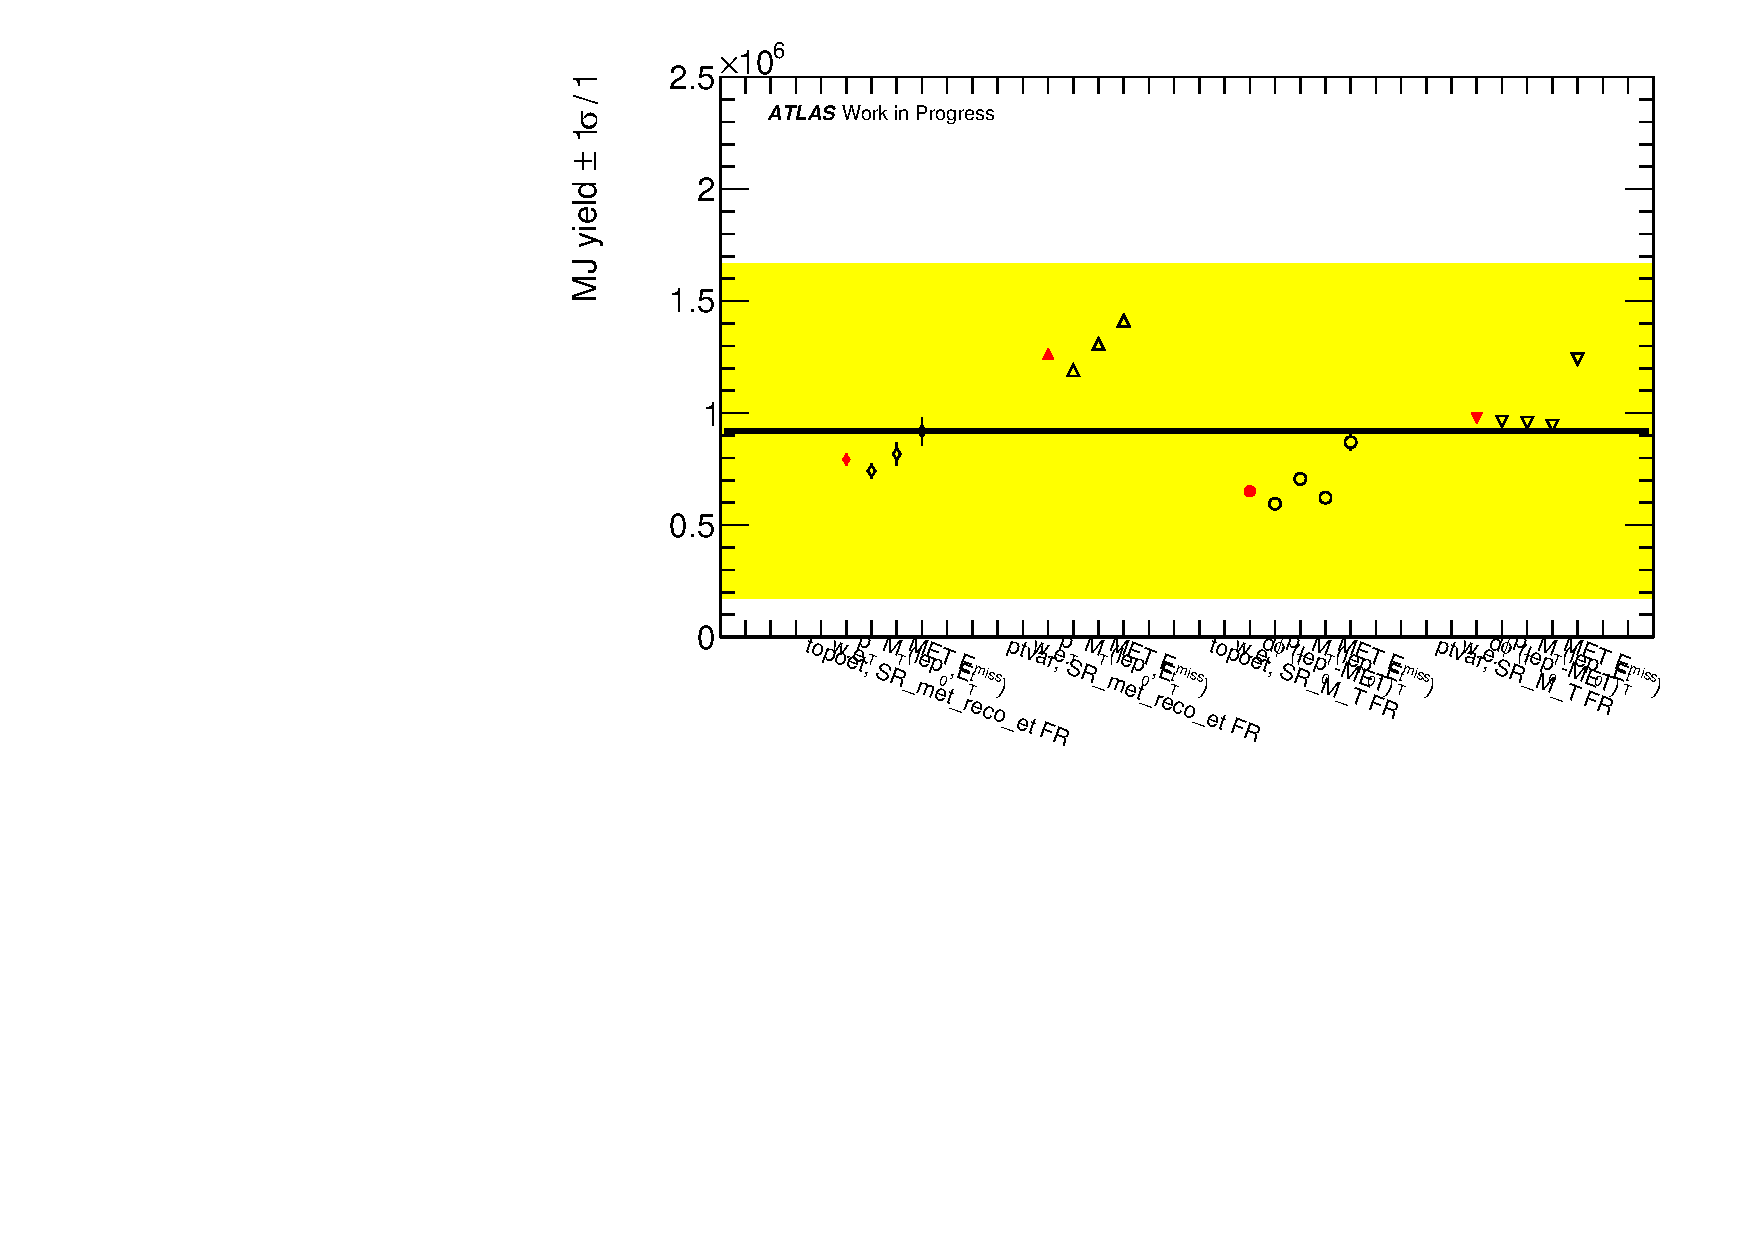
\includegraphics[width=0.75\textwidth]{figures/mj/spread_mj_el.pdf}
\caption{
 The spread of the extrapolations from each scan and their errors is illustrated with black empty markers, in comparison with their weighted averages, shown with red full markers, and the final MJ estimated yield (solid black line) and total uncertainty (yellow band), for each isolation scan variable, and fit region.
}
\label{fig:mj_spread_extrapolations}
\end{figure}

\subsubsection{$W\rightarrow\mu\nu$ scan results}
\label{sec:bkg_mj_wmu_scan}

As discussed in Sec. \ref{sec:bkg_mj_approach}, the events passing the gradient isolation cut and the selection are confined in the region of ptvarcone30/$p_T$ < 0.11 and topoetcone20/$p_T$ < 0.09. 
For this reason scans on the two variables, after inverting the gradient isolation, are performed for the values reported in Table \ref{tbl:bkg_mj_wmu_scan}. 
As for the electron channel, the scans in topoetcone20/$p_T$ are performed for a fixed range of ptvarcone30/$p_T$, so that the two sets of scans are orthogonal, the details are reported in Table \ref{tbl:bkg_mj_wmu_scan}.

\begin{table}[htbp]
\small
\begin{center}
 \begin{tabular}{ | c | c | c | } 
 \hline
 Scan variable & ptvarcone30/$p_T$ & topoetcone20/$p_T$ \\
 \hline 
 Fixed cut & topoetcone20/$p_T$ < 0.09 & ptvarcone30/$p_T$ < 0.11  \\
 \hline 
 Scan starting point & 0.11 & 0.09 \\
 Slice width & 0.11 & 0.44 \\
 Number of slices & 4 & 5 \\
 \hline 
\end{tabular}
\caption{
Width of scan slices and boundaries used for $W\rightarrow \mu\nu$ channel.
}%
\label{tbl:bkg_mj_wmu_scan}
\end{center}
\end{table}

The results for the scans, separated for the two variables and two fit regions, are shown in Fig.\ref{fig:mj_extrapolation_wmunu} for $W\rightarrow e\nu$ channel.
The errors on each of the scan points are the errors from the template fit, taking into account the discrimination power of the variables, as well as the statistics of the MJ template, multiplied by the $\sqrt(\chi^2/NDoF)$, to account for eventual mismodelling in the considered variables.
More details on the extraction of the numbers are reported in Appendix \ref{sec:details_on_multijet_background_estimate_in_the_Wmunu_channel}.

\begin{figure}[htbp]
\centering
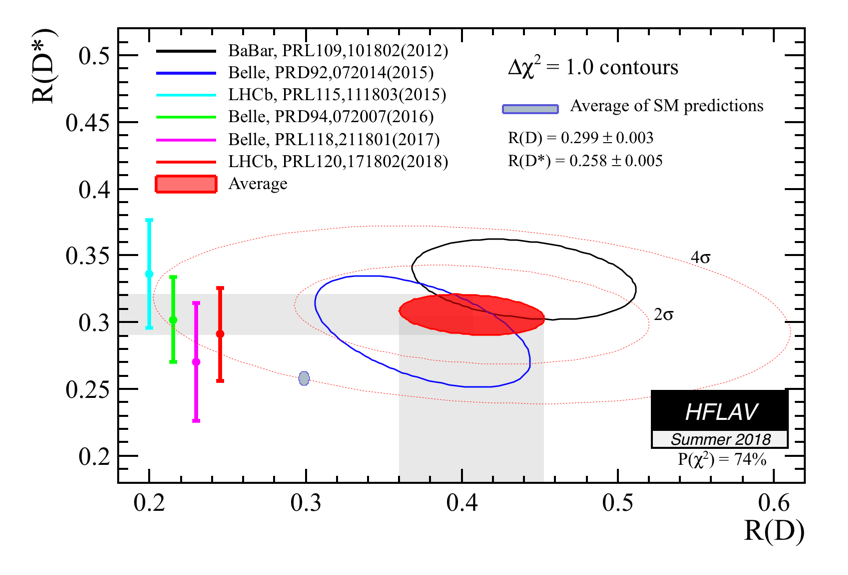
\includegraphics[width=0.45\textwidth]{figures/intro/rdrds_summer18.png}
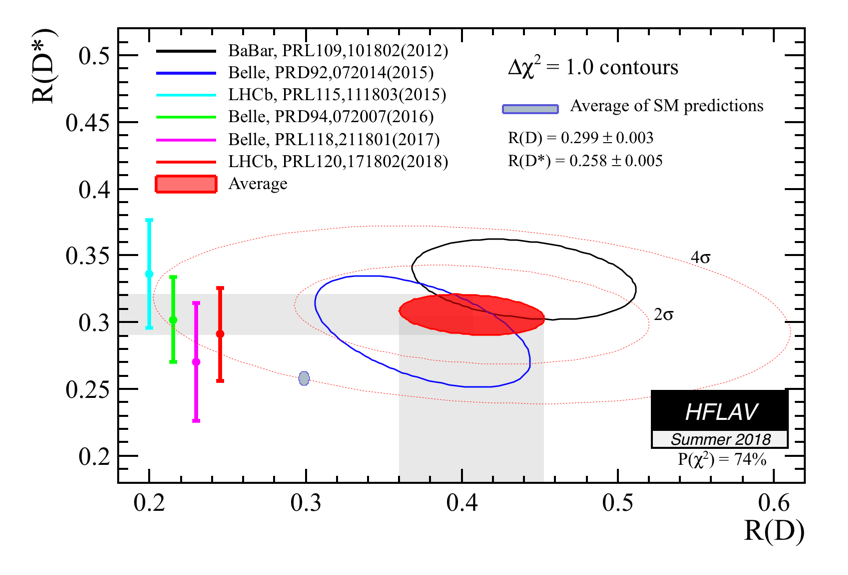
\includegraphics[width=0.45\textwidth]{figures/intro/rdrds_summer18.png}
\\
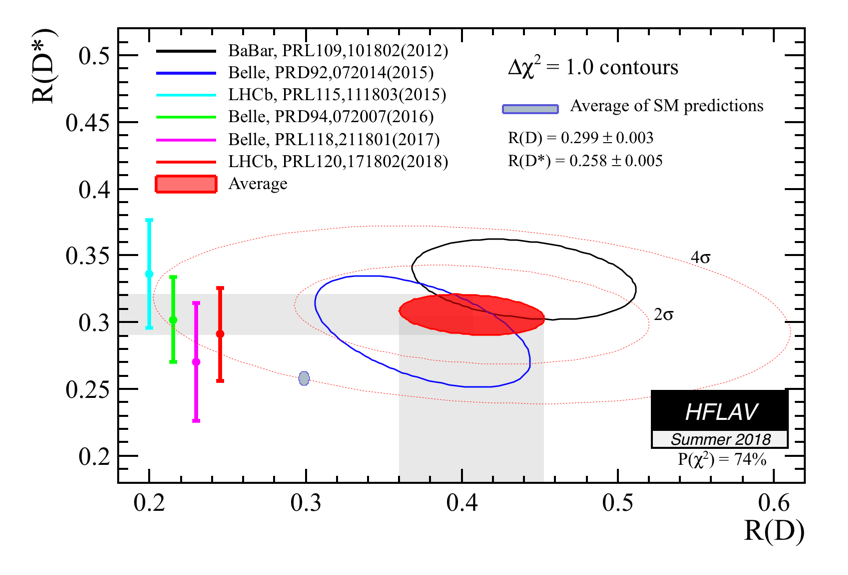
\includegraphics[width=0.45\textwidth]{figures/intro/rdrds_summer18.png}
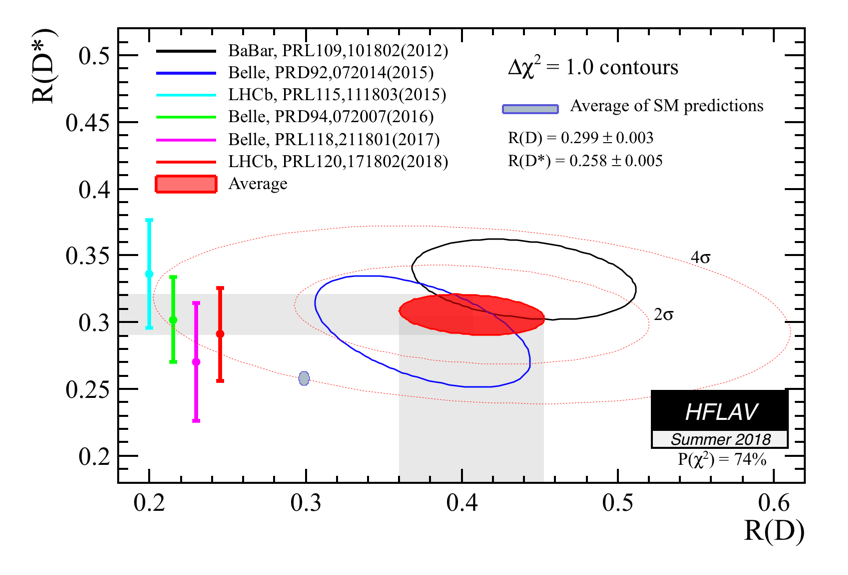
\includegraphics[width=0.45\textwidth]{figures/intro/rdrds_summer18.png}
\caption{
 Plots of the scans for ptvarcone30/$p_T$ (left column) and topoetcone20/$p_T$ (right column) for the $W\rightarrow \mu\nu$ channel, $m_T$-FR (top raw), $E_T^{miss}$-FR (bottom row).
 The results relative to the scans of the different variables (fit in each slice and linear extrapolations) are shown in different colours: $E_T^{miss}$ (blue), $m_T$ (green), $p_T$ (red) and $\Delta\varphi_{\mu,E_T^{miss}}$ (black).
%  Notice that the $\Delta\varphi_{\mu,E_T^{miss}}$ variable is missing $E_T^{miss}$-FR scans because returning often nonphysical negative or zero MJ yiels because of the poor discrimination power of such variable after the $m_T$>40 GeV cut is applied.
 The errors on each of the scan points are the error from the template fit multiplied by the $\sqrt(\chi^2/NDoF)$.
}
\label{fig:mj_extrapolation_wmunu}
\end{figure}

The SR point of extrapolation is extracted from the average value of the ptvarcone30/$p_T$ and topoetcone20/$p_T$ distributions passing the gradient isolation selection cut in data (X and Y average of top right subfigure of Figure \ref{fig:isolation_2D}).
These values are \todo{0.045} and \todo{0.03} respectively.
The extrapolated values for $W\rightarrow e\nu$ for the topoetcone20/$p_T$ and ptvarcone20/$p_T$ respectively are reported in Table \ref{tbl:bkg_mj_wmu_scan_topoet} and \ref{tbl:bkg_mj_wmu_scan_ptvar}, together with the $\chi^2/NDoF$ for the linear extrapolations.
The errors quoted come from the extrapolation at the SR points, \todo{varying in an anti-correlated way} the $p_0$ and $p_1$ liner fit parameters of one $\sigma$.

\begin{table}[htbp]
\scriptsize
\begin{center}
 \begin{tabular}{ c | c  c | c  c } 
 \hline
Fit variable & MJ extrapolated SR\_met\_reco\_et-FR & $\chi^{2}$/NDoF of linear fit & MJ extrapolated SR\_M\_T-FR & $\chi^{2}$/NDoF of linear fit \\
\hline
\multicolumn{5}{c}{$W \rightarrow \mu \nu$} \\
 \hline
 \hline 
\end{tabular}
\caption{
Results of the extrapolation to the $W\rightarrow \mu\nu$ signal region (topoetcone20/$p_T$ = \todo{0.03}). 
The errors quoted come from the extrapolation at the SR points, varying in an anti-correlated way the $p_0$ and $p_1$ linear fit parameters of one $\sigma$.
}%
\label{tbl:bkg_mj_wmu_scan_topoet}
\end{center}
\end{table}

\begin{table}[htbp]
\scriptsize
\begin{center}
 \begin{tabular}{ c | c  c | c  c } 
 \hline
Fit variable & MJ extrapolated SR\_met\_reco\_et-FR & $\chi^{2}$/NDoF of linear fit & MJ extrapolated SR\_M\_T-FR & $\chi^{2}$/NDoF of linear fit \\
\hline
\multicolumn{5}{c}{$W \rightarrow \mu \nu$} \\
 \hline
 \hline 
\end{tabular}
\caption{
Results of the extrapolation to the $W\rightarrow \mu\nu$ signal region (ptvarcone30/$p_T$ = \todo{0.045}). 
The errors quoted come from the extrapolation at the SR points, varying in an anti-correlated way the $p_0$ and $p_1$ linear fit parameters of one $\sigma$.
}%
\label{tbl:bkg_mj_wmu_scan_ptvar}
\end{center}
\end{table}

The final background yield and its systematic uncertainty are estimated from the spread of the extrapolated curves at 0.045 and 0.03 value of the ptvarcone30/$p_T$ and topoetcone20/$p_T$ variables.
To obtain the central value of the estimate, the weighted averages of the extrapolated values are computed, separately for the topoetcone and ptvarcone scans, and each fitting region.
The weighted average is calculated taking into account as anti-correlated the uncertainties on the $p_0$ and $p_1$ parameters of the fitted lines.
The nominal MJ yield is taken as the average between the four weighted averages (from the different scan variables and FR’s), and is shown in Table \ref{tbl:bkg_mj_wmu_wa_total}.
Seven sources of uncertainties, detailed in Table \ref{tbl:bkg_mj_wmu_wa_total}, are considered on the method:
\begin{itemize}
\item four come from the weighted average calculation, and are reported in Table \ref{tbl:bkg_mj_wmu_wa_extrapolation};
\item one represents the difference between the choice of scan variables, averaged over FR;
\item one represents the difference between the choice of FR, averaged over the scan variable;
\item one shows the \todo{impact of the JES variation on the signal template} in the estimated MJ yield.
\end{itemize}

\begin{table}[htbp]
\scriptsize
\begin{center}
 \begin{tabular}{ | c | c | c | c | c | } 
 \hline
Channel & \multicolumn{4}{|c|}{Weighted averages} \\
  & SR\_met\_reco\_et-FR, topoet Isol & SR\_met\_reco\_et-FR, ptvar Isol & SR\_M\_T-FR, topoet Isol & SR\_M\_T-FR, ptvar Isol \\
\hline
 
  \hline
\end{tabular}
\caption{
Weighted average for $W\rightarrow \mu\nu$ in the two channels, for both scans and fit-regions (FR), with errors coming from the extrapolation.
}%
\label{tbl:bkg_mj_wmu_wa_extrapolation}
\end{center}
\end{table}

\begin{table}[htbp]
\scriptsize
\begin{center}
 \begin{tabular}{ | c | c | c | c | c | c | c | c | } 
\hline
Channel & \textbf{MJ yield} & \multicolumn{6}{|c|}{Systematic uncertanty} \\
 &  & $E_T^{miss}$-FR, topoet & $E_T^{miss}$-FR, ptvar & $m_T$-FR, topoet & $m_T$-FR, ptvar & scan choice & FR choice \\
\hline

  \hline
\end{tabular}
\caption{
MJ estimated yield, obtained from averaging the weighted averages from the different scan variables and fit regions, and systematic uncertainties taken into account. 
The errors come from the extrapolations first four, the choice of scan variable, the choice of fit region, and \todo{shape variations} of the signal due to reconstruction systematics.
}%
\label{tbl:bkg_mj_wmu_wa_total}
\end{center}
\end{table}


\subsection{Treatment of correlations between $W^+$ and $W^-$ multijet estimates}
\label{sec:bkg_mj_WplusWminus}